\documentclass{article}
%\usepackage{fullpage}
\usepackage{fancyhdr}
\usepackage[english,francais]{babel}
\usepackage[T1]{fontenc}
\usepackage[utf8]{inputenc}
\usepackage[pdftex]{graphicx}
\usepackage{subfig}

%\renewcommand{\baselinestretch}{2}
\author{Florent \textsc{Guiotte} et Frédéric \textsc{Becker}}
\title{Filtrage}
\pagestyle{fancy}

\begin{document}
\maketitle
\tableofcontents

\section{Introduction}

Dans le cadre de ce TP, nous avons implémenté plusieurs algorithmes de filtrage, afin d'obtenir les contours
d'une image. 
Dans un premier temps nous avons implémenté les filtres gaussien et moyenneur, puis nous avons fait les détection
de contours à l'aide du filtre de Sobel et du filtre Laplacien. 

Dans les parties suivantes de ce TP, nous avons travaillé avec les images de test visibles en figure \ref{fig:croix} et
\ref{fig:calend} page \pageref{fig:init}.

\begin{figure}[!ht]%htp]
  \centering
  \subfloat[croix.pgm]{\label{fig:croix}
\includegraphics[width=0.18\textwidth]{img/croix/out.png}}
  \hspace{0.030\textwidth}
  \subfloat[calen0.pgm]{\label{fig:calend}
\includegraphics[width=0.78\textwidth]{img/calend/out.png}}
  \caption{Images de test pour les filtres de ce TP}
  \label{fig:init}
\end{figure}

\section{Lissage et rehaussement}
\subsection{Filtre séparable}

Pour réaliser le filtre gaussien, nous avons utilisé la séparabilité du filtre. On décompose le filtre pour
pouvoir faire un filtrage monodimensionnel sur les lignes puis sur les colonnes de l'image. Cette méthode est plus
rapide à l'éxecution qu'un filtrage bidimensionnel avec un filtre de taille $n\times n$. Séparabilité du filtre
gaussien~:

\begin{equation}
\left[ \begin{array}{ccc}
        1 & 2 & 1 \\
        2 & 4 & 2 \\
        1 & 2 & 1 \end{array} \right] 
    =
 \left[ \begin{array}{c}
        1\\
        2\\
        1 \end{array} \right] 
    \times
 \left[ \begin{array}{ccc}
        1 & 2 & 1 \end{array} \right] 
\end{equation}

Le resulat du filtre gaussien est visible figure \ref{gauss:init} page \pageref{gauss:init}.

\begin{figure}[!ht]%htp]
  \centering
  \subfloat[croix.pgm]{\label{gauss:croix}
\includegraphics[width=0.18\textwidth]{img/croix/gaussien.png}}
  \hspace{0.030\textwidth}
  \subfloat[calen0.pgm]{\label{gauss:calend}
\includegraphics[width=0.78\textwidth]{img/calend/gaussien.png}}
  \caption{Filtrage gaussien}
  \label{gauss:init}
\end{figure}

Nous avons fait la même manipulation avec le filtre moyenneur. Par comparaison des résultat sur les images, le filtre gaussien conserve mieux les
contours.

\subsection{Rehaussement de contours}

On applique le réhaussement avec et sans filtrage gaussien (filtre passebas). Les résultats sont visibles figure
\ref{rehauss:init}.
Le prétraitement avant le réhaussement des contours permet d'atténuer les zones moins contrastés avant d'accuentuer les
contours.
\begin{figure}[!ht]%htp]
  \centering
  \subfloat[Réhaussement simple]{\label{rehauss:base}
\includegraphics[width=0.48\textwidth]{img/croix/rehaussement.png}}
  \hspace{0.030\textwidth}
  \subfloat[Prétraitement puis réhaussement]{\label{rehauss:pb}
\includegraphics[width=0.48\textwidth]{img/croix/passsebas_rehaussement.png}}
  \caption{Filtre de réhaussement des contours}
  \label{rehauss:init}
\end{figure}

\section{Détection de contours}
\subsection{Filtre de Sobel}
Comme prétraitement à ce filtre, on peut utiliser un filtre passe bas (gaussien) affin de gommer les imperfections de
l'image
(on ne veut garder que les contours des objets idéalement).

Le filtre de Sobel est directionnel, si on l'applique à l'horizontal et à la vertical, les résultats sont visibles
figures \ref{sobel:h} et \ref{sobel:v}.

\begin{figure}[!ht]%htp]
  \centering
  \subfloat[Filtre de Sobel horizontal]{\label{sobel:h}
\includegraphics[width=0.48\textwidth]{img/calend/sobelh.png}}
  \hspace{0.030\textwidth}
  \subfloat[Filtre de Sobel vertical]{\label{sobel:v}
\includegraphics[width=0.48\textwidth]{img/calend/sobelv.png}}
  \caption{Filtre passe haut de Sobel}
  \label{rehauss:init}
\end{figure}

Pour obtenir les contours à la fois horizontaux et verticaux, on peut additionner les deux images obetnues puis
seuiller le résultat. La valeur du seuil détermine ce qui différencie le contour d'un objet du bruit de l'image.
Le résultat est visible figure \ref{sobelc:init}.


\begin{figure}[!ht]%htp]
  \centering
  \subfloat[croix.pgm]{\label{sobelc:croix}
\includegraphics[width=0.18\textwidth]{img/croix/sobel_contour.png}}
  \hspace{0.030\textwidth}
  \subfloat[calen0.pgm]{\label{sobelc:calend}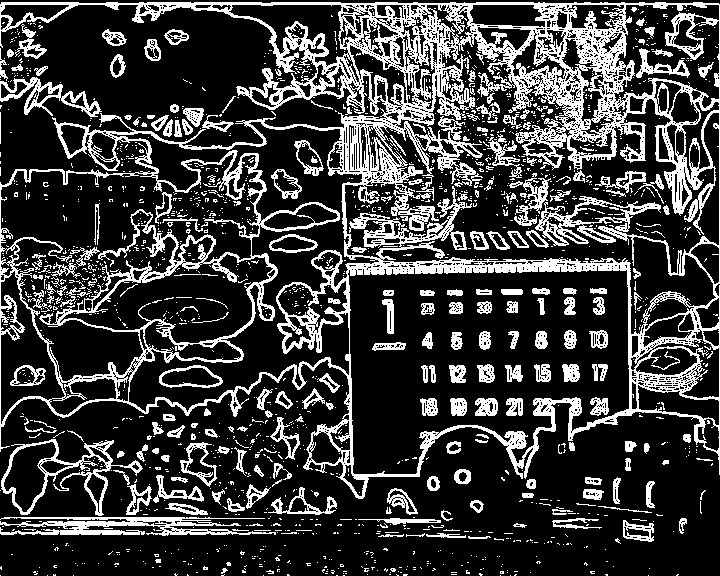
\includegraphics[width=0.78\textwidth]{img/calend/sobel_contour.png}}
  \caption{Détection de contour avec filtre de Sobel}
  \label{sobelc:init}
\end{figure}

\subsection{Filtre Laplacien}

Comme Sobel, ce filtre permet d'obtenir les contours d'une image. Nous avons choisi d'utiliser la version non séparable
du filtre laplacien de
\textsc{Prewitt}. Après le décalage des valeurs pour rendre le résultat visible dans une image classique, on obtiens le
rendu visible figure \ref{laplace:init}.

\begin{figure}[!ht]%htp]
  \centering
  \subfloat[croix.pgm]{\label{laplce:croix}
\includegraphics[width=0.18\textwidth]{img/croix/laplacien.png}}
  \hspace{0.030\textwidth}
  \subfloat[calen0.pgm]{\label{laplace:calend}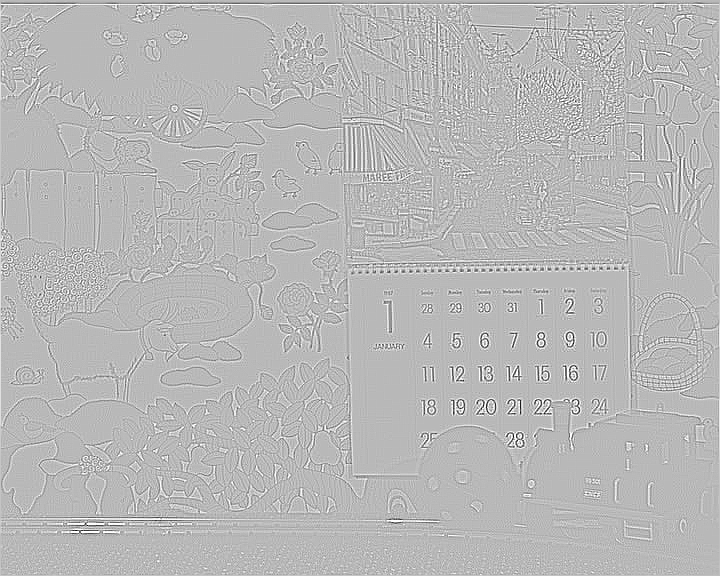
\includegraphics[width=0.78\textwidth]{img/calend/laplacien.png}}
  \caption{Filtre Laplacien}
  \label{laplace:init}
\end{figure}

La détection des contours se fait par le passage par zéro du laplacien. Ce calcul nécessite aussi un seuil d'une valeur
arbitraire pour différencier les objets du bruit. Le résultat est visible figure \ref{laplacec:init}.

\begin{figure}[!ht]%htp]
  \centering
  \subfloat[croix.pgm]{\label{laplcec:croix}
\includegraphics[width=0.18\textwidth]{img/croix/laplacien_contour.png}}
  \hspace{0.030\textwidth}
  \subfloat[calen0.pgm]{\label{laplacec:calend}
\includegraphics[width=0.78\textwidth]{img/calend/laplacien_contour.png}}
  \caption{Détection de contour à l'aide du filtre Laplacien}
  \label{laplacec:init}
\end{figure}

\section{Conclusion}
La détection de contour à l'aide du filtre de Sobel donne de meilleurs résultats.
La détection du passage par zéro du filtre Laplacien n'est pas optimal, les contours sont beaucoup plus discontinus et
pourtant la valeur du seuil les fait apparaitre plus épais que les contours de Sobel.


%\begin{figure}[!ht]
%    \center
%    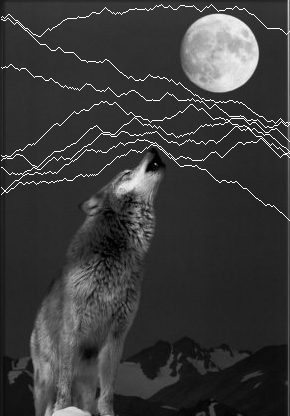
\includegraphics[width=0.48\textwidth]{img/seams.png}
%    \caption{Coutures d'énergie minimales}
%    \label{seams}
%\end{figure}

\end{document}
